\chapter{Ray tracing}\label{chap:raytracing}
Ray tracing is a geometric problem that describes the transport of light within optical systems.
It uses single rays to describe the propagation of light through an optical system.
The influence of diffraction on the transport of a ray is neglected and geometrical modeling of an optical system is considered.
Generally, the method can be implemented for two or more dimensions and for any optical system.
In the following a description of the ray tracing method  in two dimensions is given.
\section{Ray tracing for two-dimensional optical systems}
Ray tracing is a procedure that can be applied to non-imaging systems. It consists of tracing each ray, which is considered to be a broken line, through the optical system.
Given a Cartesian coordinate system $(\variabile{x}, \variabile{z})$, a two-dimensional optical system symmetric with respect to the $\variabile{z}$-axis is defined.
The optical system is formed by a source \point{S}, a target  \point{T} and some optical components $\lineai$ where $\lineai \in \{2, \cdots, \nline-1\}$ and $\nline$
 indicates the number of lines that form the system. \point{S} and \point{T} are indicated with the indexes $1$ and $\nline$, respectively. 
The index of refraction of the medium in which line $\lineai$ is located is indicated with $\n_\lineai$
Every ray emitted by \point{S} (line $1$) can hit some optical components $\lineai\in\{2, \cdots \nline -1\}$ before reaching the target $\nline$. 
The intersection point of the rays with line $\lineai$ are $(\variabile{x}_\lineai, \variabile{z}_\lineai)_{\lineai =1, \cdots, \nline}$ and, $\vect{s}_\lineai= (-\sin \optangle_\lineai, \cos \optangle_\lineai)$ indicates the direction vector of the rays that leave $\lineai$,
with $\optangle_\lineai$ the angle that the ray forms with respect to the \variabile{z}-axis measured counterclockwise. As we consider only forward rays, the angles 
$\optangle_\lineai\in (-\pi/2, \pi/2)$.
%From now on, the coordinates $(\variabile{x}_{\variabile{i}}, \variabile{z}_{\variabile{i}})_{\variabile{i} =1, \cdots, 4}$ denote the intersection of the rays with line $\variabile{i}$ and,
Therefore, a ray segment between $(\variabile{x}_\lineai, \variabile{z}_\lineai)$ and $(\variabile{x}_\lineaj, \variabile{z}_\lineaj)$ 
with $\lineaj\neq\lineai$ is parameterized in real space by:
\begin{equation}
\label{parametrization}
\vect{r}(\variabile{s})=
\left( \begin{array}{cc}
\variabile{x}_\lineai-\variabile{s}\sin(\optangle_\lineai) \\
\variabile{z}_\lineai+\variabile{s}\cos(\optangle_\lineai)\end{array} \right) \qquad \quad 0\leq \variabile{s}\leq \variabile{s}_{\textrm{max}}\,,
\end{equation}
where \variabile{s} denotes the arc-length and $\variabile{s}_{\textrm{max}}$ is the maximum value that it can assume. 
To make clear the notation, in Fig. we show an example where a single ray is traced inside a very simple optical system, the so-called two-faceted cup. 
\begin{figure}[h]
\label{figure:cup}
  \begin{center}
  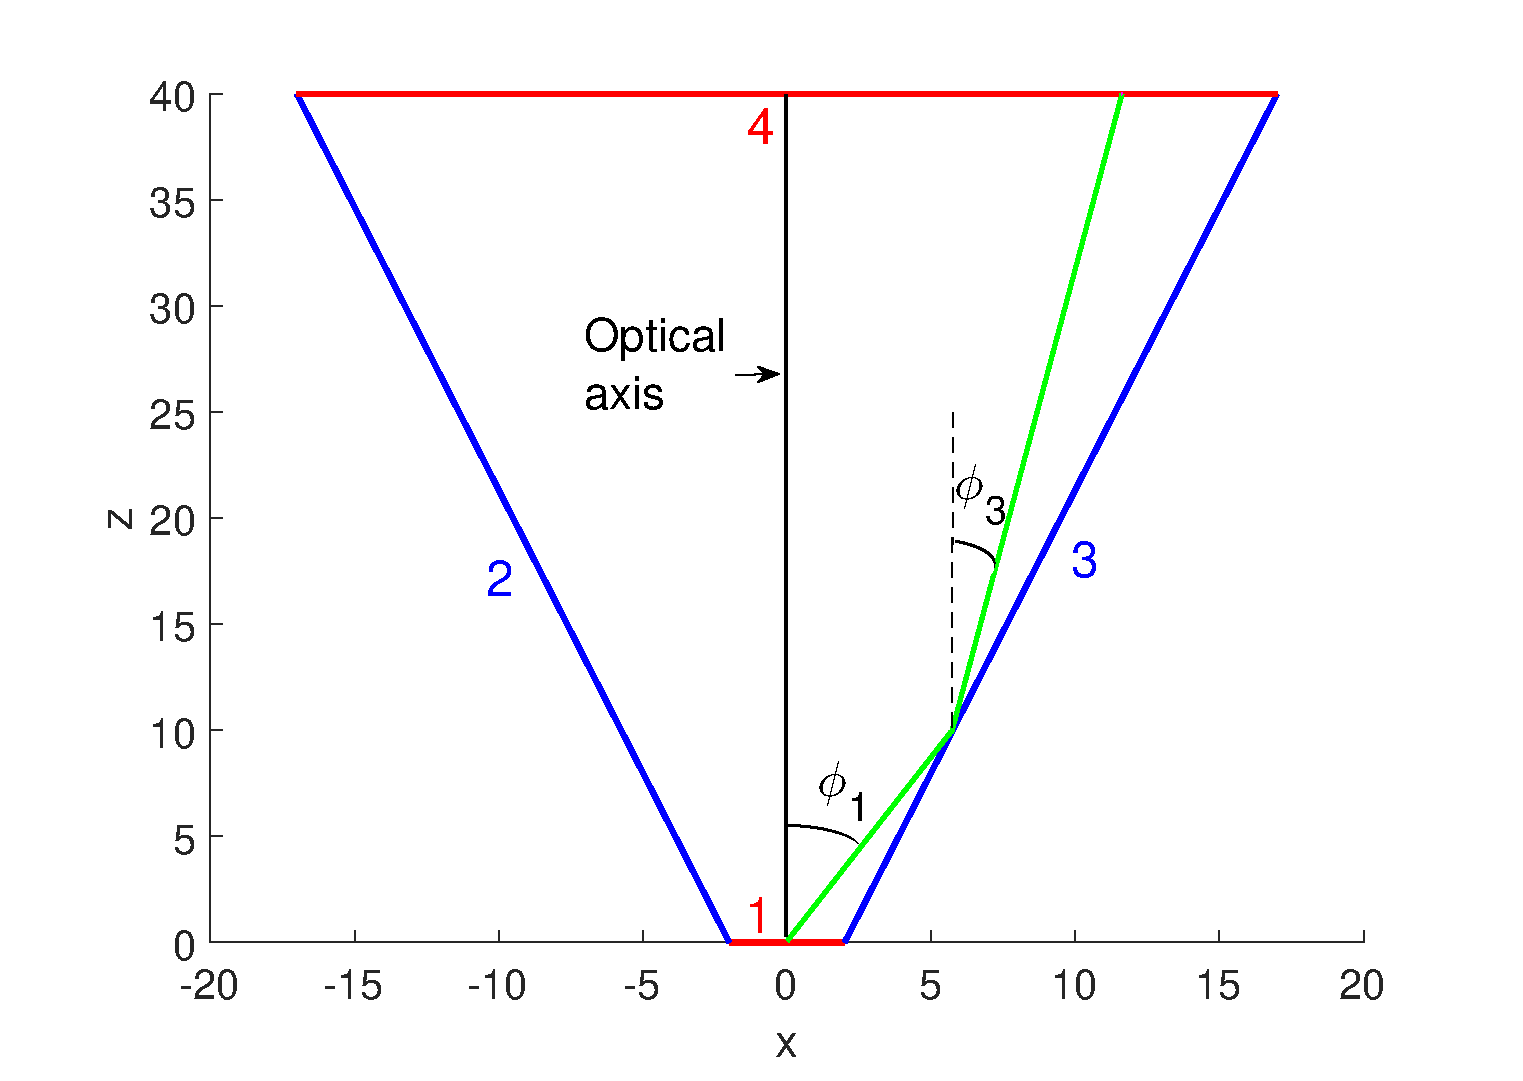
\includegraphics[width=6.7cm]{cup}
  \end{center}
  \caption{\footnotesize{Shape of the two-faceted cup.  Each line of the system is labeled with a number.
   The source \point{S}$= [-2,2]$ (line number $1$) is located on the $x$-axis.
   The target \point{T}$= [-17, 17]$ (line $4$) is parallel to the source and is located at a height $ z= 40$.
   The left and right reflectors (line $2$ and $3$) connect the source with the target.}}
  \label{figure:cup}
\end{figure}
The light source \point{S}$= [-\variabile{a}, \variabile{a}]$ (line $1$) and the target \point{T}$~=~ [-\variabile{b}, \variabile{b}]$ (line $4$) are two segments normal to the \variabile{z}-axis, where $\variabile{a}=2$ and $\variabile{b}=17$.
The left and right reflectors (line $2$ and $3$) are oblique segments that connect the source and the target.
All the optical lines $\lineai \in \{1, \cdots, 4\}$  are located in air, therefore the refractive index $\n_{\lineai}=1$ for every $\lineai$.  
\section{Monte Carlo ray tracing}
Assuming a Lambertian source, the input intensity at $\point{S}$ emitted in the direction $\variabile{t}_1$ is given by:
\begin{equation}\label{lambertian_source}
I(\variabile{t}_1) = 2\const{a}L\cos(\variabile{t}_1),
\end{equation}
where $L$ is the luminance and \variabile{a} is the half width of \point{S}.
In order to compute the target intensity, we need to find a relation between the intensities at \point{S} and \point{T}.
 Hence, we need to know how the optical system influences the direction of the rays when they hit an optical line.
 To this purpose, the ray tracing procedure is often used in optics.
Ray tracing relates the position coordinates
 $ (\variabile{x}_1, \variabile{z}_1)$ and the direction vector $\vect{s}_1$ of every ray at the source $\point{S}$ with the corresponding position $(\variabile{x}_4, \variabile{z}_4)$ and direction $\vect{s}_4$
 at the target $\point{T}$. As in the following we will use often the target coordinates of the rays, from now on, to simplify the notation, we write $\variabile{t}$ instead of $\variabile{t}_4$ and $(\variabile{x}, 
\variabile{z})$ instead of $(\variabile{x}_4, \variabile{z}_4)$ for the target coordinates.\\ \indent The ray tracing algorithm can be schematized as follows.
 For every ray that leaves $\point{S}$ with initial position $(\variabile{x}_1, \variabile{z}_1)$ and initial angle $\variabile{t}_1$, its ray parametrization is implemented according to Eq. ($\ref{parametrization}$). 
Then, the coordinates $(\variabile{x}_\variabile{i}, \variabile{z}_\variabile{i})$ of the intersection point between the ray and the line $\variabile{i}$ that it hits are computed. The unit normal 
$\boldsymbol{\nu}_\variabile{i}$ to the line $\variabile{i}$ at the point $(\variabile{x}_{\variabile{i}}, \variabile{z}_{\variabile{i}})$ is calculated to compute the change of direction of the ray.
 Since all the lines of the system are located in air, only the reflection law plays a role, \cite{Hecht}.
 Therefore, denoting with $\vect{t}_1$ the direction of the incident ray, the direction $\vect{t}_2$ of the reflected ray is given by:
 \begin{equation}\label{reflection}
  \vect{t}_{2} = \vect{t}_1-2(\vect{t}_1,\boldsymbol{\nu}_{\variabile{i}})\boldsymbol{\nu}_{\variabile{i}}\,,
\end{equation}
where the vectors $\vect{t}_{1}$ and $\vect{t}_{2}$ are unit vectors, \cite{Chaves}.
The procedure explained above is repeated for every line that the ray encounters until it reaches the target and for every ray traced through the system. \\ \indent
There are different ways to implement the ray tracing procedure.
An often used method is MC ray tracing which calculates the target photometric variables considering a sample of many rays that are traced randomly from $\point{S}$ to $\point{T}$. The output intensity is computed as a 
function of the angular coordinate $\variabile{t}$ and is calculated dividing the target into intervals of the same length, the so-called bins. A partitioning 
$P_1: -\pi/2 = \variabile{t}_{0}<\variabile{t}_{1}<\cdots <\variabile{t}_{\const{Nb}}=\pi/2$ of the interval $[-\pi/2, \pi/2]$ is defined where $\const{Nb}$ is the number of bins in $P_1$.
We remark that, with a slight abuse of notation, we indicated the angular coordinates of the rays at the target with $\variabile{t}_{\variabile{j}}$ instead of $\variabile{t}_{4,\variabile{j}}$ for every $\variabile{j}\in\{0, \cdots, \const{Nb}\}$.
The normalized approximated intensity $g_{\const{MC}}(\variabile{t})$ is a piecewise constant function and its value over the $\variabile{j}$-th bin is the ratio between the number of rays that fall into that bin
$\const{Nr}[\variabile{t}_{\variabile{j}-1},\variabile{t}_{\variabile{j}})$ and the total number of rays traced $\const{Nr}[-\pi/2, \pi/2]$.
Hence, $g_{\const{MC}}$ is defined by:
\begin{equation} \label{g_mc}
g_{\const{MC}}(\variabile{t}) = \frac{\const{Nr}[\variabile{t}_{\variabile{j}-1},\variabile{t}_{\variabile{j}})}{\const{Nr}[-\pi/2, \pi/2]} \qquad \mbox{ for } \variabile{t}\in[\variabile{t}_{\variabile{j}-1}, \variabile{t}_{\variabile{j}}).
\end{equation}
Furthermore, the output intensity is computed from the value of the intensity $g_{\const{MC}}(\variabile{t}_{\variabile{j}-1/2})$ along the direction $\variabile{t}_{\variabile{j}-1/2}=(\variabile{t}_{\variabile{j}-1}+
\variabile{t}_{\variabile{j}})/2$ for every bin $[\variabile{t}_{\variabile{j}-1},\variabile{t}_{\variabile{j}})_{\variabile{j} = 1, \cdots, \const{Nb}}$.
 The intensity $g_{\const{MC}}(\variabile{t}_{\variabile{j}-1/2})$ gives an estimate of the probability that a ray reaches the target with an angle in the $\variabile{j}$-th interval 
$[\variabile{t}_{\variabile{j}-1}, \variabile{t}_{\variabile{j}})$ of the partitioning $P_1$. This probability $\const{P}_{\variabile{j}, \Delta\variabile{t}}$ is given by:
\begin{equation}\label{eq:probability}
\const{P}_{\variabile{j}, \Delta\variabile{t}} = \Pr(\variabile{t}_{\variabile{j}-1}\leq\variabile{t}<\variabile{t}_{\variabile{j}})= 
\frac{\int_{\variabile{t}_{\variabile{j}-1}}^{\variabile{t}_{\variabile{j}}} G(\variabile{t}) \textrm{d}\variabile{t}}{\int_{-\pi/2}^{\pi/2}G(\variabile{t}) \textrm{d}\variabile{t}}\,,
\end{equation}
where $G(\variabile{t})$ is the output intensity (not normalized) and it is measured in lumen per radian $[lm/rad]$.
Note that $\sum_{\variabile{j}=1}^{\const{Nb}}\const{P}_{\variabile{j}, \Delta\variabile{t}}=1$. Using the mean value theorem for the function 
$G(\variabile{t})$ continuous in $[\variabile{t}_{\variabile{j}-1}, \variabile{t}_{\variabile{j}}]$, the integral at the numerator of the previous equation can be written as: \begin{equation}
\int_{\variabile{t}_{\variabile{j}-1}}^{\variabile{t}_{\variabile{j}}} G(\variabile{t}) \textrm{d}\variabile{t} = \Delta \variabile{t}\;G(\variabile{t}_{j-1/2}).
\end{equation}
Hence, $\const{P}_{\variabile{j}, \Delta\variabile{t}}$ is proportional to the size $\Delta\variabile{t}= (\variabile{t}_{\const{Nb}}-\variabile{t}_{0})/{\const{Nb}}$ 
of the intervals, i.e., inversely proportional to the number of bins $\const{Nb}$ of the partitioning $P_1$.
Indicating with $\Phi = \int_{-\pi/2}^{\pi/2}G(\variabile{t}) \textrm{d}\variabile{t}$ the total flux (measured in lumen $[lm]$),
the error between the intensity $G(\variabile{t}_{\variabile{j}-1/2})$
 and the averaged \const{MC} intensity $\Phi g_{\const{MC}}(\variabile{t}_{\variabile{j}-1/2})/\Delta\variabile{t}$ is given by:
\begin{equation}\label{eq:error_int}
\begin{aligned}
\Big|G(\variabile{t}_{\variabile{j}-1/2})&-\frac{\Phi}
{\Delta\variabile{t}}g_{\const{MC}}(\variabile{t}_{\variabile{j}-1/2})\Big| \leq\\
 &\Big|G(\variabile{t}_{\variabile{j}-1/2})-\frac{1}{\Delta \variabile{t}}\int_{\variabile{t}_{\variabile{j}-1}}^{\variabile{t}_{\variabile{j}}} G(\variabile{t})\textrm{d}\variabile{t}\Big|+\\
&\frac{1}{\Delta \variabile{t}}\Big|\int_{\variabile{t}_{\variabile{j}-1}}^{\variabile{t}_{\variabile{j}}} G(\variabile{t})\textrm{d}\variabile{t}-
\Phi\, g_{\const{MC}}(\variabile{t}_{\variabile{j}-1/2})\Big| \,.
\end{aligned}
\end{equation}
\indent The first term of the right hand side of inequality (\ref{eq:error_int}) gives an estimate of how much the averaged intensity
 $\frac{1}{\Delta \variabile{t}}\int_{\variabile{t}_{\variabile{j}-1}}^{\variabile{t}_{\variabile{j}}} G(\variabile{t})\textrm{d}\variabile{t}$ differs from the exact intensity $G(\variabile{t}_{\variabile{j}-1/2})$.
This term is due to the discretization of the target and therefore it depends on the number of bins $\const{Nb}$ considered.
  Substituting $G(\variabile{t})$ with its Taylor expansion around the point $\variabile{t}_{\variabile{j}-1/2}$ we obtain that this term is proportional to the square of the size of the bins, therefore the following equality holds:
\begin{equation}\Big|G(\variabile{t}_{\variabile{j}-1/2})-\frac{1}{\Delta \variabile{t}}\int_{\variabile{t}_{\variabile{j}-1}}^{\variabile{t}_{\variabile{j}}} G(\variabile{t})\textrm{d}\variabile{t}\Big| = \const{C}_1/\const{Nb}^2\end{equation}
with $C_1>0$ a certain constant. \\
\indent
The second part of the right hand side of inequality (\ref{eq:error_int}) gives an estimate of the MC error and therefore it depends also on the
number of rays traced.
In order to show how this term decreases as a function of the number of rays traced,
we define the random variable $\variabile{X}_\variabile{j}(\variabile{t})$ as the variable that is equal to $1$ if the ray with angular coordinate $\variabile{t}$
is inside the interval $[\variabile{t}_{\variabile{j}-1}, \variabile{t}_{\variabile{j}})$ and equal to $0$ otherwise,
\begin{equation}
\label{radom_variable}
\variabile{X}_{\variabile{j}}(\variabile{t}) = \begin{cases} \begin{aligned}
1& \qquad \mbox{if} \quad \variabile{t}\in [\variabile{t}_{\variabile{j}-1}, \variabile{t}_{\variabile{j}}),\\
0 & \qquad \mbox{otherwise}.
\end{aligned}\end{cases}
\end{equation}
The Bernoulli trial $ \variabile{X}_{\variabile{j}}$ follows a binomial distribution $B(1,\const{P}_{\variabile{j}, \Delta\variabile{t}})$.
Considering a sample of $\const{Nr}$ rays, the variable $\variabile{Y}_{\variabile{j}} = \sum_{\variabile{k}=1}^{\const{Nr}} \variabile{X}_{\variabile{j}}(\variabile{t}_{\variabile{k}})$
follows a binomial distribution $B(\const{Nr}, \const{P}_{\variabile{j},\Delta \variabile{t}})$, where $\variabile{t}_{\variabile{k}}$ is the angle that the $\variabile{k}$-th ray forms
 with the optical axis. Then, using the de Moivre-Laplace theorem, we conclude that the variable $\variabile{Y}_{\variabile{j}}$ is approximated by a normal distribution with mean value 
$\variabile{E}[\variabile{Y}_{\variabile{j}}] = \const{Nr}\const{P}_{\variabile{j}, \Delta\variabile{t}}$ and variance $\sigma^2[\variabile{Y}_{\variabile{j}}] = \const{Nr}\const{P}_{\variabile{j}, \Delta\variabile{t}}(1~-~\const{P}_{\variabile{j}, \Delta\variabile{t}})$ 
when a large number of rays is considered, see \cite{Rubinstein, deMoivre}.
Thus, the normalized intensity along the direction $\variabile{t}_{\variabile{j}-1/2}$ is given by:
\begin{equation}\variabile{g}_{\const{MC}}(\variabile{t}_{\variabile{j}-1/2}) = \sum_{\variabile{k}=1}^{\const{Nr}}\variabile{X}_{\variabile{j}}(\variabile{t}_{\variabile{k}})/\const{Nr}.\end{equation}
The mean value $E[\variabile{g}_{\const{MC}}(\variabile{t}_{\variabile{j}-1/2})]=\const{P}_{\variabile{j}, \Delta\variabile{t}}$
and the variance $\sigma^2[\variabile{g}_{\const{MC}}(\variabile{t}_{\variabile{j}-1/2})] ~=~ \const{P}_{\variabile{j}, \Delta\variabile{t}}(1-\const{P}_{\variabile{j}, \Delta\variabile{t}})/\const{Nr}$.
Note that the standard deviation $\sigma_\variabile{j}:=\sigma[\variabile{g}_{\const{MC}}(\variabile{t}_{\variabile{j}-1/2})]$ equals:
\begin{equation}\label{sigma}
\sigma_\variabile{j}= \sqrt{\const{P}_{\variabile{j}, \Delta\variabile{t}}(1-\const{P}_{\variabile{j}, \Delta\variabile{t}})/\const{Nr}}= \frac{\const{C}_2}{\sqrt{\const{Nb}\const{Nr}}}\,, \end{equation}
 for some $\const{C}_{2}>0$. $\sigma_\variabile{j}$ can be used to give an estimate of the difference between the intensity $\variabile{g}_{\const{MC}}(\variabile{t}_{\variabile{j}-1/2})$ and its mean value $\const{P}_{\variabile{j}, \Delta\variabile{t}}$.
Therefore, the second term of the right hand side of relation ($\ref{eq:error_int}$) becomes:
\begin{equation}\begin{aligned}
\frac{1}{\Delta \variabile{t}}\Big|\int_{\variabile{t}_{\variabile{j}-1}}^{\variabile{t}_{\variabile{j}}} G(\variabile{t})\textrm{d}\variabile{t} -
\Phi\, g_{\const{MC}}(\variabile{t}_{\variabile{j}-1/2})\Big| &=  \\
\frac{\Phi}{\Delta \variabile{t}}\Big|\const{P}_{\variabile{j}, \Delta\variabile{t}} -g_{\const{MC}}(\variabile{t}_{\variabile{j}-1/2})\Big| &\propto  \\
  \frac{\Phi}{\Delta \variabile{t}}
\sigma_{\variabile{j}}[\variabile{g}_{\const{MC}}(\variabile{t}_{\variabile{j}-1/2})]=\const{C}_3\frac{\const{Nb}}{\sqrt{\const{Nb}\const{Nr}}} & = \const{C}_3\sqrt{\frac{\const{Nb}}{\const{Nr}}}\,,
\end{aligned}
\end{equation}
for some $\const{C}_3>0$, where the approximation holds because $\sigma_{\variabile{j}}$ gives a measure for the error between 
$g_{\const{MC}}(\variabile{t}_{\variabile{j}-1/2})$ and the probability $\const{P}_{\variabile{j}, \Delta\variabile{t}}$, \cite{Diez}. The second equality follows from Eq. (\ref{sigma}). To conclude, the MC error over the $\variabile{j}$-th bin is estimated by:
\begin{equation} \begin{aligned}
\Big|G(\variabile{t}_{\variabile{j}-1/2})&-\frac{\Phi}
{\Delta\variabile{t}}g_{\const{MC}}(\variabile{t}_{\variabile{j}-1/2})\Big| =
\frac{\const{C}_1}{\const{Nb}^2} + \const{C}_4\sqrt{\frac{\const{Nb}}{\const{Nr}}},
\end{aligned}
\end{equation}
for $\const{C}_4>0$.
Considering a fixed number of rays, we obtain that the minimal error is reached when $\const{Nb}\approx \const{Nr}^{1/5}$.
Hence, if $10^{10}$ rays are considered the target has to be divided into $10^2$ bins to minimize the MC error.
This leads to computational efforts resulting in a very slow procedure.





To obtain the photometric variables at the target, the propagation of light from the source $\mathcal{S}$ to the target $\mathcal{T}$ is computed.
In this work, we calculate the output intensity for the TIR-collimator, the profile of which is depicted in Figure $\ref{fig:analyticlens}$.
\begin{figure}[t]
  \begin{center}
  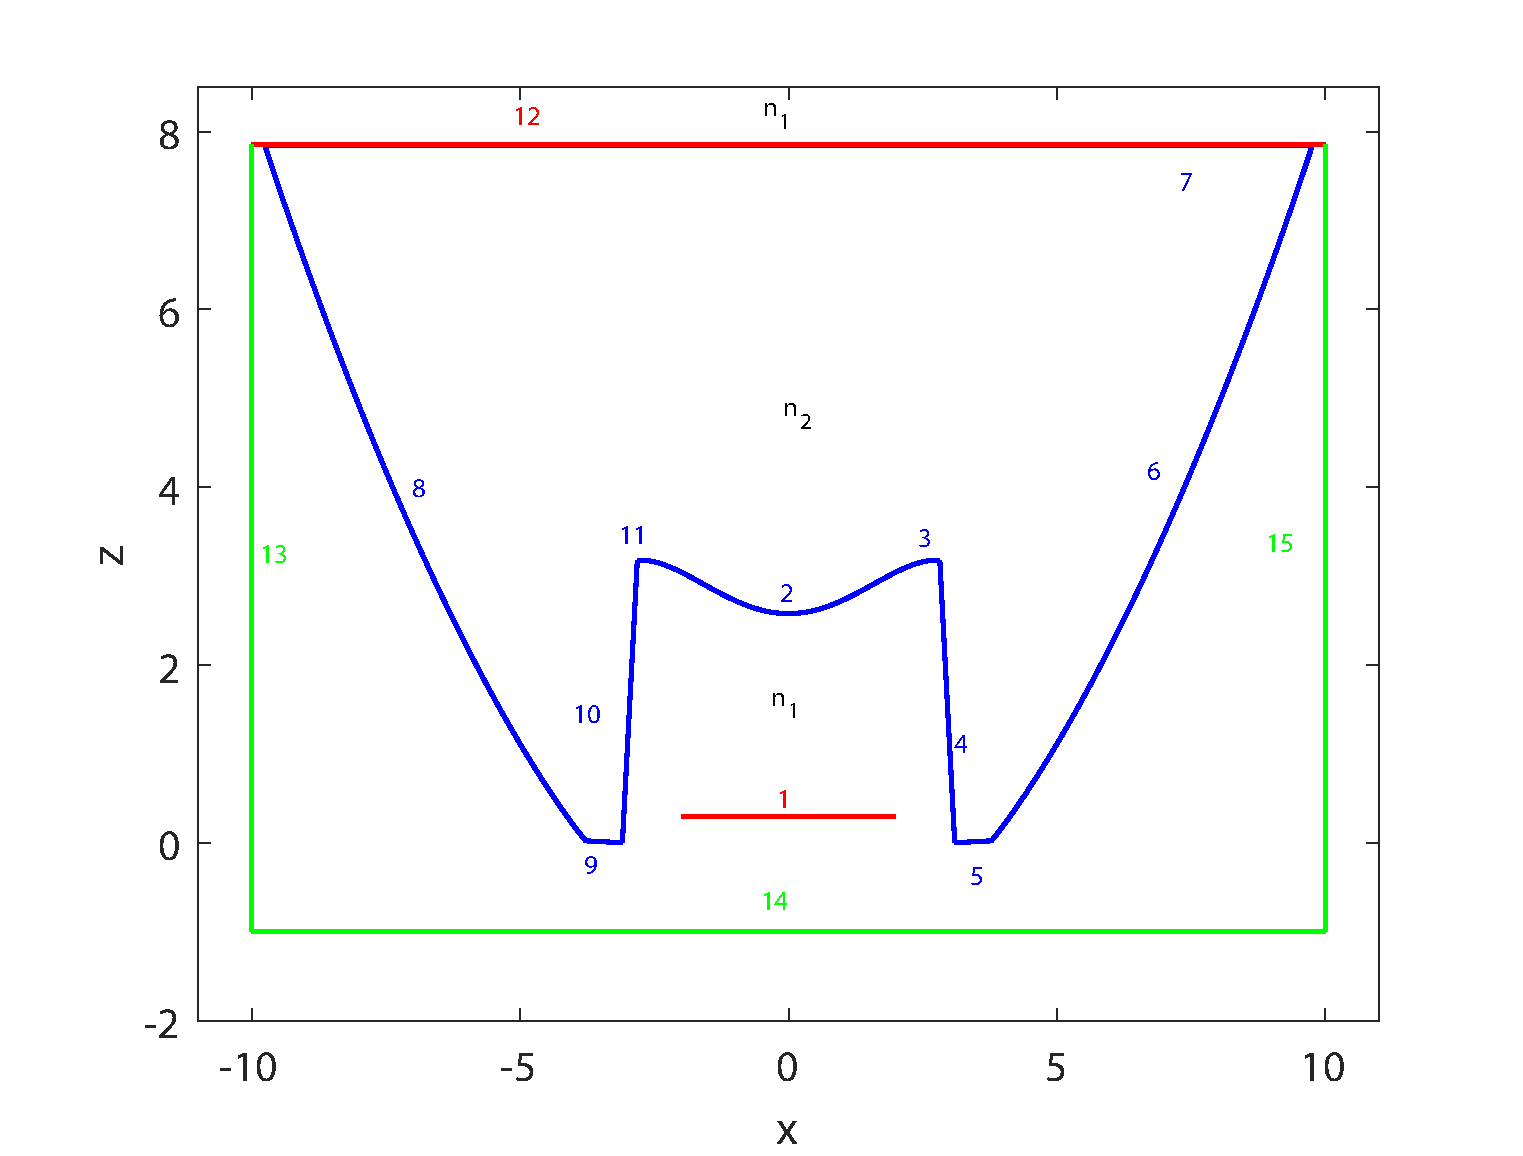
\includegraphics[width=6.5cm]{tir_analytic2.pdf}
   \end{center}
    \caption{\footnotesize{Shape of the TIR-collimator. Each line of the system is labeled with a number.
       The source $\mathcal{S}= [-2,2]$ (line number $1$) is located at an height $z_{\textrm{s}} = 0.3$ from the $x$-axis.
       The target $\mathcal{T}= [-9.7, 9.7]$ (line $12$) is parallel to the source and is located at an height $ z_{\textrm{t}}= 7.85$.
       The shape of the collimator is shown as a blue line.
       Three detectors depicted with green lines (lines $13$, $14$, and $15$) are located at the left, the right and the bottom of the optical system.
       $n_1 = 1$ is the refraction index of the medium (air) where the source and the target are located, and
       $n_2 = 1.5 $ the refraction index of the medium (glass) inside the optical system. The sagitta of the lens is equal to $0.6$.}}
 \label{fig:analyticlens}
\end{figure}
\\
The TIR-collimator we analyze is an optical system rotationally symmetric with respect to the $z$-axis and consists of a lens (line $2$), two broken lines adjacent to the lens (formed by the collection of the segments $3, 4, \mbox{ and } 5$ and $9, 10 \mbox{ and } 11$),
two curved lines (labeled with $6$ and $8$) and the top formed by a horizontal segment (line $7$). The lens and the broken lines are refractive lines while, the curved lines are designed in such a way that light is internally reflected (which explains the name TIR).
The light source $\mathcal{S}$ (line $1$) and the target $\mathcal{T}$ (line $12$) are two straight segments normal to the optical axis and are located in air ($n_1=1$) while
the volume inside the collimator is filled with a material with index of refraction $n_2=1.5$ (e.g. glass).
The collimator is surrounded by two vertical and two horizontal lines (lines $13$, $15$, $12$ and $14$, respectively) that receive the light exiting from the optical system; among these, the horizontal one at the top is assumed to be the light target and, it is located at a small distance from the top. \\
\indent From now on, the coordinates $(x_{\textit{i}}, z_{\textit{i}})_{(i =1, \cdots, 15)}$ denote the intersection of the rays with the line $\textit{i}$ and, $\textbf{s}_\textit{i}= (-\sin t_\textit{i}, \cos t_\textit{i})$ is the direction vector of the rays that leave the line $\textit{i}$, where $t_\textit{i}~\in~ (-\pi/2, \pi/2)$ is the angle
 that the ray forms with the $z$-axis, measured counterclockwise.
 Therefore, a ray segment between $(x_\textit{i}, z_\textit{i})$ and $(x_\textit{i+1}, z_\textit{i+1})$ is parameterized by:
\begin{equation}
\label{parametrization}
\textbf{r}(s)=\begin{pmatrix}x_\textit{i}-s\sin(t_\textit{i})\\ z_\textit{i}+s\cos(t_\textit{i})\end{pmatrix}  \qquad \quad s\geq 0\,,
\end{equation}
where $s$ denotes the arc-length.
\\  \indent A Lambertian optical source is considered; hence, the intensity over an interval $J ~=~ [-a, a]$ emitted in the direction $t$ is given by:
\begin{equation}
\label{lambertian_source}
I(t) = I_0\cos(t),
\end{equation}
where $I_0= 2aL$, $L$ is the luminance, and $t$ is the angle that the ray forms with respect to the optical axis, measured counterclockwise.
As a result, in the case where $L=1$, $I_0$ coincides with the source length; from Equation ($\ref{lambertian_source}$), the intensity at the source is deduced. \\
\indent To compute the target intensity, we need to know how the optical system changes the direction of the rays during their propagation from the source to the target.
To do this, we employ the ray tracing technique which can be summarized as follows: first, a ray from the source with initial position given by the coordinates $(x_1, z_1)$ and initial angle $t_1$ with respect to the $z$- axis is traced and, the ray parametrization is implemented according to Equation ($\ref{parametrization}$). Second, the intersection point $(x_\textit{i}, z_\textit{i})$ between the ray and the line $\textit{i}$ that it hits first is computed. Third, the normal to the line hit at the point $(x_{\textit{i}}, z_{\textrm{i}})$ is calculated to compute the change of direction of the ray.
For the last step, the laws of reflection and refraction are implemented.
The direction of the refractive ray is given by:
\begin{equation}\label{refraction}
\textbf{t}=n_{1,2}\,\textbf{i}+\Big[\sqrt{1-n_{1,2}^2+n_{1,2}^2(\textbf{n},\textbf{i})^2}-n_{1,2}(\textbf{n},\textbf{i}) \Big]\textbf{n}\,,
\end{equation}
where $n_{1,2}=n_1/n_2$ with $n_1$ and $n_2$ the refraction indexes of air and of glass, respectively.
The unit vectors $\textbf{i}$ and $\textbf{t}$ describe the directions of the incident and refracted ray, respectively; $\textbf{n}$ is the normal to the line; it is also a unit vector and it is directed towards the interior of the optical system.
Note that the positive sign before the square root is due to the convention to take the inward direction of the normal $\textbf{n}$ (see \cite{hecht1998hecht}, chapter 4, p. 95-106, and, \cite{chaves2008introduction}, chapter 12 p. 403-409).
In the case where $n_1 = -n_2$, Equation (\ref{refraction}) can be rewritten as the law of reflection:
\begin{equation}\label{reflection}
\textbf{t} = \textbf{i}-2(\textbf{i}, \textbf{n})\textbf{n}.
\end{equation}
Equation ($\ref{reflection}$) is used when the total internal reflection condition holds, that is when the following inequality is true:
\begin{equation}\label{eq: Tir-condition}
1-n_{1,2}^2+(\textbf{n},\textbf{i})^2<0\,.
\end{equation}
For the TIR-collimator the previous condition occurs for the curved lines (lines $6$ and $8$ in Figure \ref{fig:analyticlens}).
Finally, the new parametrization of the ray is described by:
\begin{equation}
\textbf{r}(s)=
\begin{pmatrix}
x_i+s\,t_{x} \\ z_i+s\,t_{z}
\end{pmatrix}\,,
\end{equation}
where
$t_{x}$ and $t_{z}$ are the $x$ and $z$-components of the new ray direction and are calculated from Equations ($\ref{refraction}$) or ($\ref{reflection}$).
The points $(x_\textit{i}, z_\textit{i})$ and the new direction $\textbf{t}$ are computed until the ray hits the target and the previous procedure is repeated for each ray traced. \\
\indent To obtain a reasonable approximation of the target intensity, a large number of rays has to be traced; the more rays are traced, the more accurate the target intensity is.
Moreover, for the TIR-collimator shown in Figure $\ref{fig:analyticlens}$, we do not have an explicit equation to describe the reflectors. Only the positions of a discrete set of points located on their curves are known.
Therefore, we use spline interpolation to obtain a good approximation of the curved lines. In addition, to calculate the intersection points between the rays and these lines, the Newton-Raphson procedure is employed. Due to all these reasons, the ray-tracing method is a very slow procedure.\\
\indent A frequently used ray tracing method in non-imaging optics is MC ray tracing \cite{Ting:1} in which the rays are emitted from a random location and at random angle. They are traced through the system until they reach the target receiver. To calculate the output intensity, the target screen is divided into bins and the frequency of the rays that arrive at each bin is considered. The intensity restricted to a certain bin is obtained by dividing the number of rays that fall into that bin by the total number of rays traced.
Although MC ray tracing is highly robust and does not require difficult calculations, it has two main disadvantages.
First, some information is lost because the flux of a ray is averaged over a bin.
Second, some parts of the target are reached by a very small fraction of rays and, consequently, the intensity is unreliable in those parts.
As a consequence, a large number of rays needs to be traced to obtain an accurate intensity making the MC method computationally expensive.
\\
\indent We provide a new method that employs the phase space representation of the optical system to avoid tracing rays where the luminance does not present any discontinuities.
Phase space ray tracing is explained in the next section.

In phase space each ray is described by its intersection point with the line it hits and the sine of the angle it forms with respect to the optical axis multiplied by the refractive index (see \cite{wolf2004geometric} chapter 2.1-2.3, \cite{rausch2014phase}, and \cite{torre2005linear} chapter 1 for details).
In the following, the phase space is considered only for the source $\mathcal{S}$ and the target $\mathcal{T}$ and for no other line of the optical system.
The rays in a two-dimensional system correspond to points with coordinates $(x,\tau)$ and $(q,\eta)$ in $\mathcal{S}$ and $\mathcal{T}$ phase space, respectively.
We have indicated the ray positions with $x$ and $q$, the angles formed with the normal with $t$ and $\theta$, the refractive indexes with $n_{\textrm{s}}$ and $n_{\textrm{t}}$, for $\mathcal{S}$ and $\mathcal{T}$, respectively and, with $\tau = n_{\textrm{s}}\sin(t)$ and $\eta = n_{\textrm{t}}\sin(\theta)$ the directions of the rays.

The rays are represented by a unique point in phase space, both for $\mathcal{S}$ and $\mathcal{T}$.
More formally, the optical phase space for the light source is defined as: \begin{equation}
\mathcal{P}_\textrm{s}=\mathcal{S}\times[-n_\textrm{s},n_\textrm{s}] .\end{equation}
The target phase space is defined as \begin{equation}\mathcal{P}_\textrm{t}=\mathcal{T}\times[-n_\textrm{t},n_\textrm{t}] .\end{equation}
The map $\mathcal{M}:\mathcal{P}_{\textrm{s}}\rightarrow\mathcal{P}_{\textrm{t}}$ which describes how the optical system changes the rays is defined as:
\begin{equation}\label{M}
\mathcal{M}(x,\tau)=(q,\eta).
\end{equation}
For most optical systems, there is no way to determine an explicit expression for the map $\mathcal{M}$ defined above.
The idea is to apply the edge-ray principle \cite{Ries:2} to a given set of rays at the source.
The principle states that to map one region from the source to the target phase space it is sufficient to map the boundaries of those regions.
Therefore, the boundaries of the source are mapped to the boundaries of the target and the regions where the luminance is different from zero are calculated.
The intensity in target phase space is defined as a function of the output luminance:
\begin{equation}\label{I(eta)}
I_{PS}(\eta) = \int_{\mathcal{T}_{\eta}} L_{\textrm{t}}(q, \eta) dq  \,,
\end{equation}
where, for a given constant $\eta_0 \in [-1,1]$, the set $\mathcal{T}_{\eta_0}~=~\{(q, \eta)~\in~ \mathcal{T}\:|\: \eta ~=~ \eta_0 \}$ and $L_{\textrm{t}}(q, \eta)$ indicates the luminance at the target.
As we use the target phase space to compute the output intensity, it is convenient to define it as a function of $\sin(\theta)$ instead of $\theta$.
Note that the luminance is positive in the entire $\mathcal{P}_\textrm{s}$, but not all parts of $\mathcal{P}_\textrm{t}$ receive light emitted by the source.
As a result, $L_\textrm{t}$ has jump discontinuities where it changes from zero to positive values.
To understand where these discontinuities occur, further information about the rays is required.
Because of this, for PS ray tracing not only the initial positions and the initial angles of the rays are stored,
 but also the optical lines they hit when they propagate through the system.
A ray path $\Pi$ is defined as the collection of lines hit by the ray. %that the rays hit when propagate through the optical system.
Rays that are close to each other at the source and leave the source at close angles follow the same path and hit the target at close positions and under close angles.
All the rays that follow the same path are grouped together into the same subset of phase space.
 From now on, we indicate with $p$ the number of all the possible paths $(\Pi_{j})_{j = 1, \cdots, p}$ encountered by the rays
  and, with $R_{\textrm{s}, \Pi_j}$ and $R_{\textrm{t}, \Pi_j}$ the regions corresponding to the rays that follow the path $\Pi_j$ for the source and the target, respectively.
  The map $\mathcal{M}$ defined in Equation (\ref{M}) relates the regions $R_{\textrm{s}, \Pi_j}$ to the regions $R_{\textrm{t}, \Pi_j}$ for every $j \in \{1, \cdots,p \}$.
The edge-ray principle guarantees that the boundaries $\partial R_{\textrm{s}, \Pi_j}$ and $\partial R_{\textrm{t}, \Pi_j}$ are connected by the same map $\mathcal{M}$.
Given two different paths $\Pi_1$ and $\Pi_2$, the regions $R_{\textrm{t}, \Pi_1}$ and $R_{\textrm{t}, \Pi_2}$ do not overlap; they can have at most a common boundary.
As a result, the discontinuities of the luminance occur exactly at the boundaries $(\partial R_{\textrm{t}, \Pi_j})_{j = 1,\cdots, p}$.
Finally, the luminance at the target satisfies the following relations:
\begin{equation}
\begin{array}{cc}
\begin{aligned}
 \label{luminance}
L_\textrm{t}(q, \eta) &> 0  &\qquad \mbox{ for } (q, \eta)\in (R_{\textrm{t}, \Pi_j})_{j = 1, \cdots, p}, \\
L_\textrm{t}(q, \eta) &= 0 &\mbox{otherwise}. \qquad \qquad \qquad \;\;\,
\end{aligned}
\end{array}
\end{equation}
In addition, the luminance is conserved along a ray, so it remains constant inside every region $ (R_{\textrm{t}, \Pi_j})_{j  =1, \cdots, p }$, (see \cite{chaves2008introduction}, chapter 16).
The output intensity is obtained from Equation ($\ref{I(eta)}$).
Therefore, the problem to compute the target intensity can be interpreted as the calculation of the boundaries $(\partial R_{\textrm{t}, \Pi_j})_{j = 1,\cdots, p}$.
To this end, we define a triangulation on source phase space in such a way that more rays close to the boundaries are traced.
The details of these procedures are explained in the next section.

\subsection{Triangulation refinement of source phase space} \label{subsec:triangulation1}
The regions $(R_{\textrm{t}, \Pi_j})_{j =1, \cdots, p}$ can be defined only when some rays are traced.
Given an initial set of rays, the rays closest to the boundaries $(\partial R_{\textrm{t}, \Pi_j})_{j = 1, \cdots, p}$ are selected and more rays in their vicinity are created to get progressively better estimates of the boundaries. A more detailed description is provided below.
A triangulation in $\mathcal{P}_\textrm{s}$ is defined and a ray from every vertex $(x_k, \tau_k)$ of the triangle is traced.
The procedure starts tracing four rays with coordinates $(x_k,\tau_k)_{k=1, \cdots, 4}$ that are located exactly at the corners of $\mathcal{P}_\textrm{s}$ and, for each of them, the paths $(\Pi_{j})_{j = 1, \cdots, 4}$, are stored. Next, for some $j \in\{1, \cdots, 4\}$, the grid is divided into two equal triangles joining two opposite vertices. For each triangle the rays located at its corners are traced. If the paths corresponding to
those rays are different, one or more boundaries
$(\partial R_{\textrm{t}, \Pi_j})_{j =1, \cdots, 4}$ are expected to cross the triangle.
In that case, the middle points $(x_k, \tau_k)_{k = 5, 6, 7}$ of each side of the triangle are added and
three more rays with coordinates $(x_k, \tau_k)_{k = 5, 6,7}$ are traced. Each refinement step leads to four new triangles (see Figure \ref{fig:refinement}).
 \begin{figure}[t]
  \begin{center}
  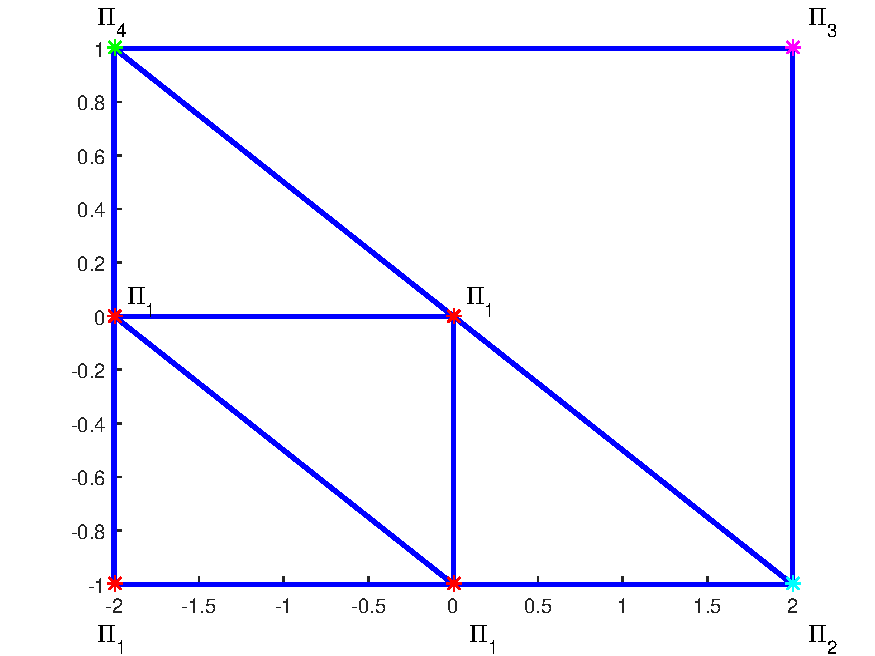
\includegraphics[width=5.7cm]{grid.pdf}
  \end{center}
  \caption{\footnotesize{Triangulation refinement:
  when the rays related to the vertices of the triangles follow a different path a new refinement step is required.
   Each refinement step leads to four new triangles.
   The parameters values are $\epsilon_{x_{max}}~=~ 2$, $\epsilon_{\tau_{max}}= 1$, $\epsilon_{x_{min}}= 4$ and $\epsilon_{\tau_{min}}=2$.   }}
  \label{fig:refinement}
\end{figure}
  \\
 \indent
When all the rays in the corners of each triangle have the same path, it is not necessary to refine the triangles anymore.
\noindent Note that it can happen that a region formed by rays that follow a path $\Pi_j$ is located completely inside a triangle whose vertices are related to the same path $\Pi_i$ with $j \neq i$. In that case the algorithm is not able to detect that region, see Figure \ref{fig:region inside}. To avoid this, two parameters $\epsilon_{x_{min}}$ and $\epsilon_{\tau_{min}}$ are defined for the $x$-axis and the $\tau$-axis, respectively. When the length of the sides of the triangle are greater than these parameters, a new triangle is defined even if its vertices correspond to the same path. Furthermore, two other parameters $\epsilon_{x_{max}}$ and $\epsilon_{\tau_{max}}$ are introduced to defined a stopping criterion.
The algorithm stops when the length of the sides of the triangles is smaller than $\epsilon_{x_{max}}$ and $\epsilon_{\tau_{max}}$.
\begin{figure}[t]
  \begin{center}
  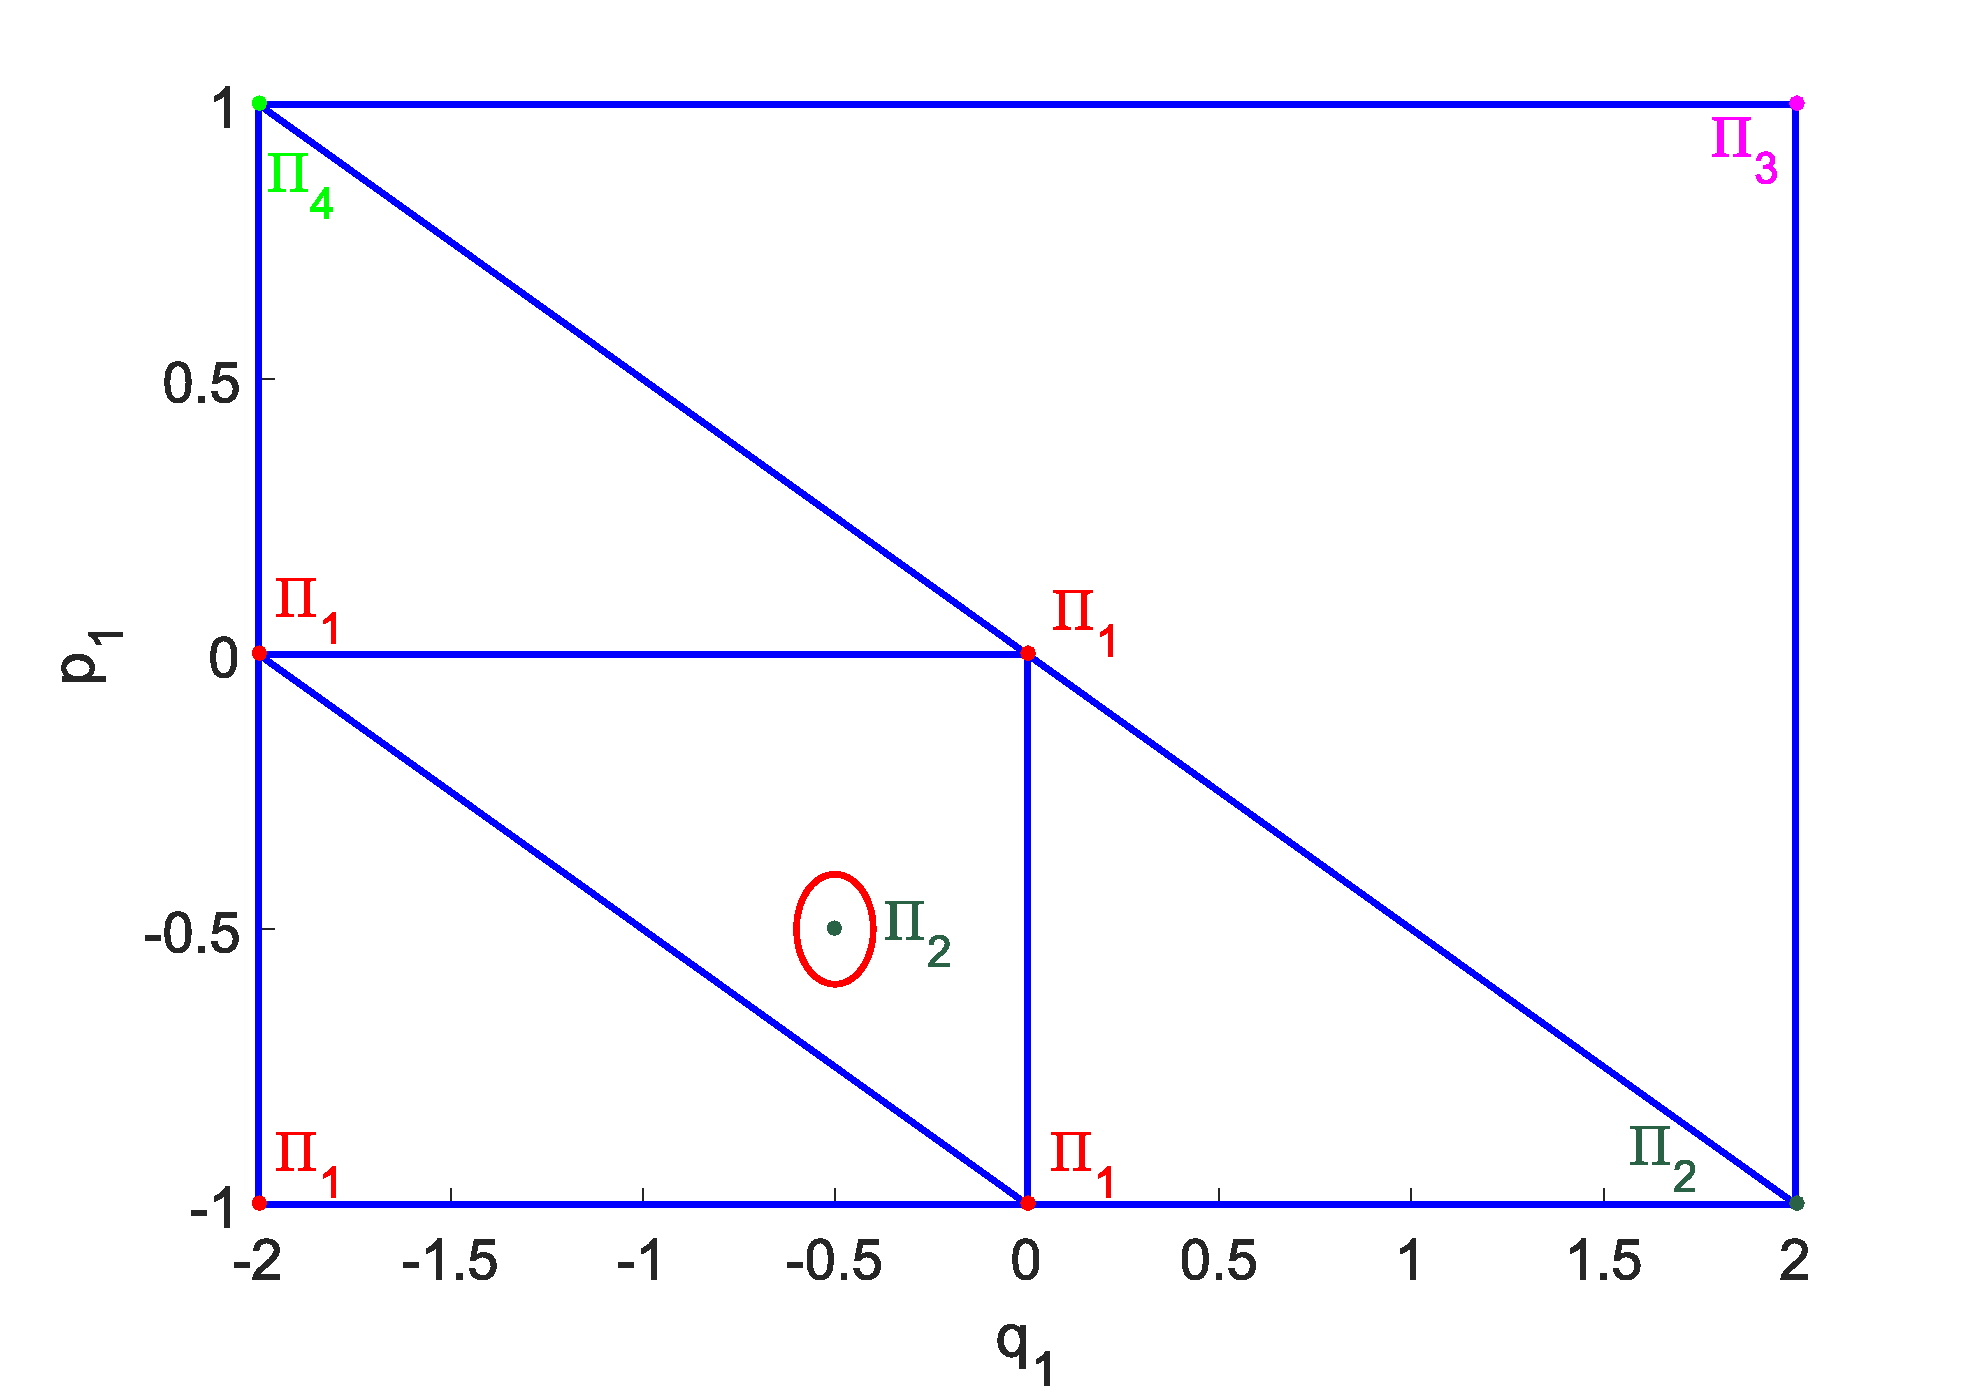
\includegraphics[width=5.5cm]{region_inside.pdf}
  \end{center}
  \caption{\footnotesize{The red line encloses a region of rays that follow the path $\Pi_2$ and is completely located inside a triangle.
  The algorithm is not able to detect that region and, a further refinement is required.
    The parameters values are $\epsilon_{x_{max}}~=~ 2$, $\epsilon_{\tau_{max}}= 1$, $\epsilon_{x_{min}}= 4$ and $\epsilon_{\tau_{min}}=2$. }}
   \label{fig:region inside}
  \end{figure}
The values of the parameters $\epsilon_{x_{max}}$, $\epsilon_{\tau_{max}}$, $\epsilon_{x_{min}}$ and $\epsilon_{\tau_{min}}$ determine the number of rays traced.
Indeed, on the one hand, $\epsilon_{x_{max}}$ and $\epsilon_{\tau_{max}}$ can be decreased to obtain more rays close to the boundaries;
on the other hand, a large number of rays in the interior of the regions can be traced decreasing the values of $\epsilon_{x_{min}}$ and $\epsilon_{\tau_{min}}$. %
\newline
\indent Using the above procedure, rays increasingly closer to the boundaries are traced.
For our optical system, the width of the $x$-axis in source phase space is two times the width of the $\tau$-axis.
Thus, our choice is $\epsilon_{\tau_{min}}=\frac{1}{2}\epsilon_{x_{min}}$ and $\epsilon_{\tau_{max}} = \frac{1}{2}\epsilon_{x_{max}}$.
Figure \ref{fig:triangulation_refinement} shows an example of a triangulation refinement of the source phase space with $\epsilon_{x_{max}}=0.1$ and $\epsilon_{x_{min}}=1$.
The triangulation refinement provides more triangles close to the boundaries $\partial R_{\textrm{s}, \Pi_j}$ than those inside the regions $R_{\textrm{s}, \Pi_j}$.
\begin{figure}[h]
  \begin{center}
  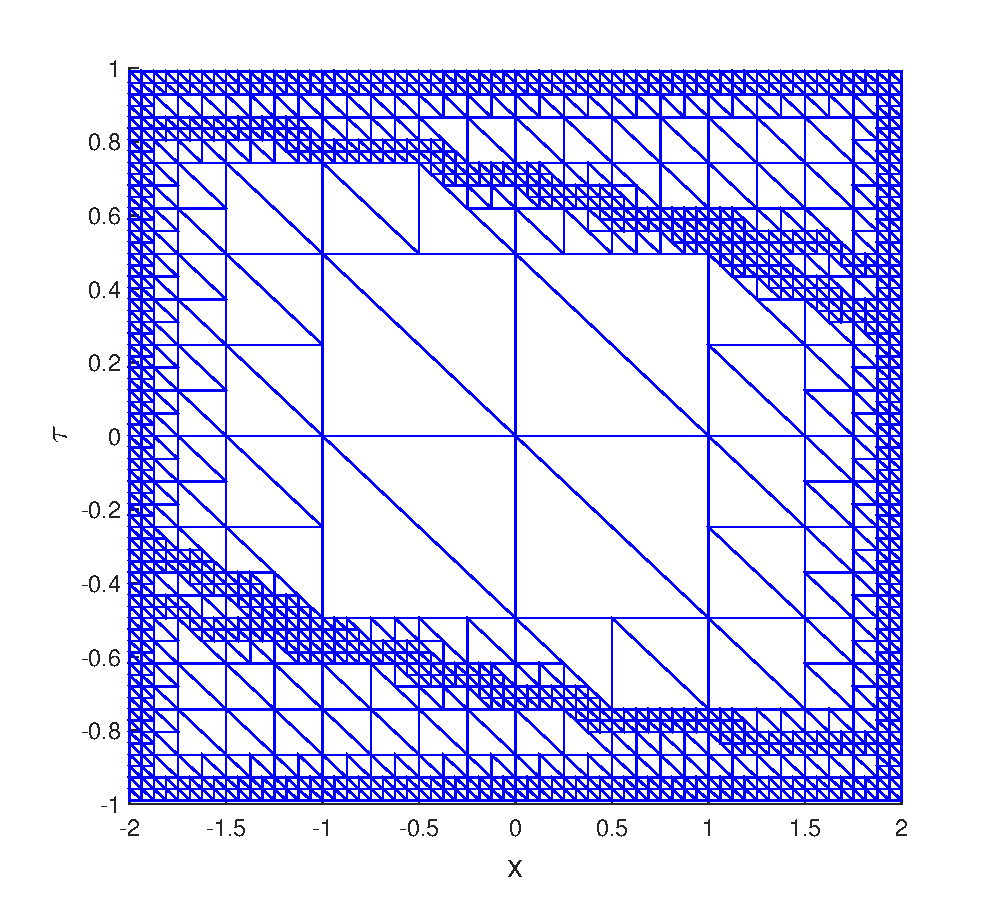
\includegraphics[width=5.7cm]{triangulation_refinement1.pdf}
  \end{center}
  \caption{\footnotesize{Triangulation refinement of source phase space:
  near the boundaries more rays are traced.
    The values of the parameters are $\epsilon_{x_{max}}~=~ 0.1$ and $\epsilon_{x_{min}}~=~1$.}}
   \label{fig:triangulation_refinement}
  \end{figure}
 \\ \indent The paths $(\Pi_j)_{j = 1, \cdots, p}$ followed by the rays located at the corner of the triangles are computed during the procedure and, the regions
 $R_{\textrm{s}, \Pi_j}$ and $R_{\textrm{t}, \Pi_j}$ are defined for each $\Pi_j$.
Next, a criterion to select the values of the parameters $\epsilon_{x_{min}}$ and $\epsilon_{x_{max}}$ and a method to compute the boundaries $\partial{R_{t, \Pi_j}}$ is provided.
Furthermore, the output photometric variables are computed, the details are explained in the next section.
As mentioned in Section \ref{sec:method}\ref{subsec:phasespace}, the boundaries $(\partial R_{\textrm{t}, \Pi_j})_{j = 1,\cdots, p}$ have to be calculated to compute the photometric variables at the target. Our method is based on the triangulation refinement of the source phase space.
More rays close to the boundaries can be traced selecting increasingly smaller values for the parameters $\epsilon_{x_{max}}$ and $\epsilon_{\tau_{max}}$. Once the algorithm stops, only the triangles that are expected to be crossed by a boundary are taken into account.
By construction, each of these triangles has two vertices that follow the same path and one vertex that follows another path.
The triangles are ordered in such a way that two of them are neighbors if they have a side in common. Given a path $\Pi_j$ with $j \in \{1, \cdots, p\}$ the boundary $\partial R_{\textrm{s}, \Pi_j}$ of the region corresponding to $\Pi_j$ is approximated by those vertices of the triangles corresponding to the path $\Pi_j$.
The boundaries $\partial R_{t, \Pi_j}$ at the target are given by $\mathcal{M}(\partial R_{s, \Pi_j})$ for every $j \in \{1, \cdots, p \}$.
To establish the minimum value of the parameter $\epsilon_{x_{max}}$ that gives a good approximation of the boundaries $\partial R_{\textrm{t}, \Pi_j}$,
a technique that exploits the conservation of the \'{e}tendue in phase space is provided, (see \cite{chaves2008introduction}, chapter 16). The essence of our approach is as follows.\\
\indent We consider the \'{e}tendue for the whole $\mathcal{P}_\textrm{s}$ which is given by:
\begin{equation}\label{etenduesource}
E_{\textrm{s}} = 2n_{\textrm{s}} a \sin(t_{max})\,,
\end{equation}
 where $a$ is the length of the source  and $t_{max}$ is the maximum value of the angle that the rays make with the $z$-axis.
 The \'{e}tendue of a set of rays is defined by the area they occupy in phase space.
 For the TIR-collimator we considered (Figure \ref{fig:analyticlens}), the area of $\mathcal{P}_\textrm{s}$ is equal to $7.92$, as $a = 4$ and $\sin(t_{max}) ~=~ 0.99$.
 The rays traced are uniformly distributed over $\mathcal{P}_\textrm{s}$, and they cover it entirely.
 \begin{figure}[h]
  \begin{center}
  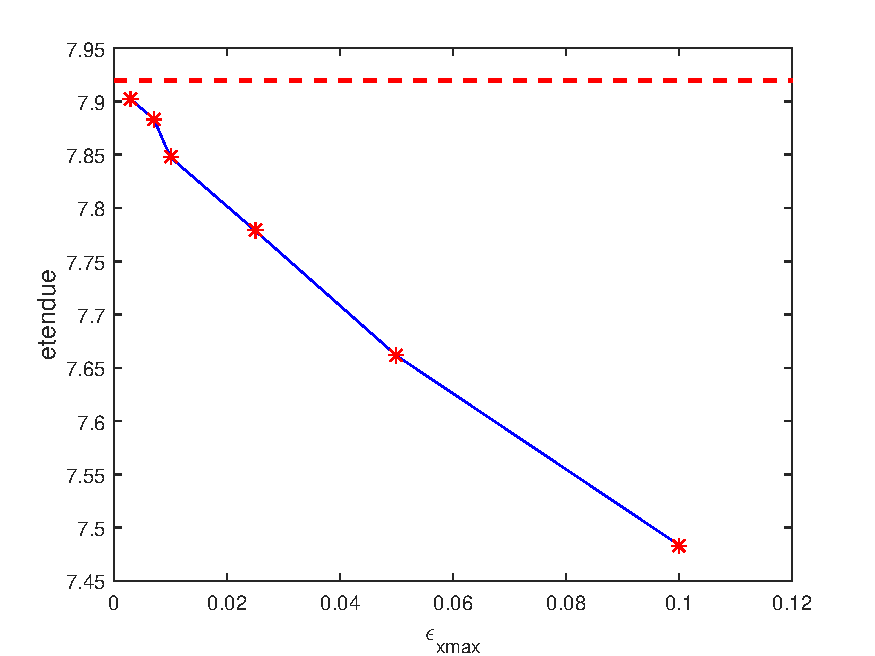
\includegraphics[width=7.7cm]{etendue.pdf}
  \end{center}
  \caption{\footnotesize{The total \'{e}tendue as an area in PS is depicted with the dotted red line. The approximated \'{e}tendue is computed for a range of values of $\epsilon_{x_{max}}$. Decreasing the value of the parameter the $\epsilon_{x_{max}}$, the \'{e}tendue increases and reaches a good approximation of the exact \'{e}tendue for $\epsilon_{x_{max}} = 3\cdot 10^{-3}$.
  }}
  \label{fig:etendueTS}
\end{figure}

 The total \'{e}tendue at the target $E_{\textrm{t}}$ is given by the sum of the \'{e}tendues related to each region $R_{\textrm{t}, \Pi_{j}}$:
 \begin{equation}
 \label{eq:etenduetarget}
 E_{\textrm{t}} = \sum_{j = 1}^p E(R_{\textrm{t}, \Pi_j})\,,
 \end{equation}
 where $E(R_{\textrm{t}, \Pi_j})$ is the contribution to the \'{e}tendue at the target given by the rays inside the region $R_{\textrm{t}, \Pi_j}$. Note that $E_{\textrm{t}}$ is computed by also considering the area of the regions formed by the rays that hit the left and the right detectors (lines $13$ and $14$ in Figure \ref{fig:analyticlens}). $E(R_{\textrm{t}, \Pi_j})$ is defined by:
  \begin{equation}\label{etenduepartial}
 E(R_{\textrm{t}, \Pi_j}) = {\int\!\!\int}_{R_{\textrm{t}, \Pi_j}} \textrm{d}q\textrm{d}\eta \,.
 \end{equation}
 To calculate the previous integral the triangulation refinement method is applied to the regions $R_{\textrm{s}, \Pi_j}$ for a range of values of $\epsilon_{x_{max}}$, with an approximation of the boundaries $\partial{R_{\textrm{s}, \Pi_j}}$ obtained for each of them.
 Therefore, the boundaries $\partial{R_{\textrm{t}, \Pi_j}}$ are also computed and the intersection points $(q_{\Pi_j,i}( \eta))_{i = 1, \cdots, r}$ between $\partial R_{\textrm{t},\Pi_j}$
and the horizontal line $\eta ~=~ const$ are calculated for each $j \in \{1, \cdots, p\}$ , with $\eta~\in~[-1,1]$. Ordering the points $(q_{\Pi_j,i}( \eta))_{i = 1, \cdots, r}$ in ascending order,
 Equation ($\ref{etenduepartial}$) becomes:
\begin{equation}
\label{eq:etenduetarg2}
 E(R_{\textrm{t}, \Pi_j}) =\sum_{i = 1}^{m} \int_{-1}^{1}{(q_{\Pi_j, 2i}( \eta)}-{q_{\Pi_j,2i-1} ( \eta) )} \textrm{d}\eta \,,
\end{equation}
where $m$ is the integer part of $r/2$ and $r$ is the number of the intersection points between $\partial R_{t,\Pi_j}$
and the horizontal lines $\eta ~=~ const$. The integral in Equation (\ref{eq:etenduetarg2}) is calculated by discretizing the interval $[-1, 1]$ into $Nb=100$ sub-intervals of equal width and using the trapezoidal rule.
Figure \ref{fig:etendueTS} shows that decreasing the value of the parameter $\epsilon_{x_{max}}$ increases the values of the \'{e}tendue at the target $E_{\textrm{t}}$, which reaches $7.9$  when $\epsilon_{x_{max}}= 0.3\cdot 10^{-3}$. We decide to stop the phase space refinement procedure when a good approximation of the \'{e}tendue is obtained.
Moreover, a criterion to establish the values of $\epsilon_{x_{min}}$ is provided.
For each value of $\epsilon_{x_{max}}$ the  \'{e}tendue for a range of values of $\epsilon_{x_{min}}$ is computed.
As the computation of the boundaries does not depend on the number of rays inside the regions, the \'{e}tendue remains constant when the value of $\epsilon_{x_{min}}$ changes. We choose $\epsilon_{x_{min}}$ as large as possible avoiding to trace rays that do not significantly contribute to the computation of the photometric variables at the target.
The value of $\epsilon_{x_{min}}$ depends on the distribution of the rays in phase space. For our optical system the parameter $\epsilon_{x_{min}}=1$.
Figure \ref{fig:sourcePS} and \ref{fig:targetPS} show the approximation of the boundaries obtained for a set of $ 6.9\cdot 10^4$ rays. Five different paths are found and rays that follow the same path are depicted with the same color. Figure \ref{fig:sourcePS} shows that, choosing the values of the parameters as explained above, the regions $R_{\textrm{s}, \Pi_j}$ almost completely cover the source phase space. As a consequence, the dark areas in Figure \ref{fig:targetPS} correspond to parts of target phase space that are not reached by any ray that leaves the source and propagates though the meridional plane of the optical system. Note that, using the triangulation procedure explained in the previous section, more rays close to the boundaries are traced.

\begin{figure}[h]
  \begin{center}
  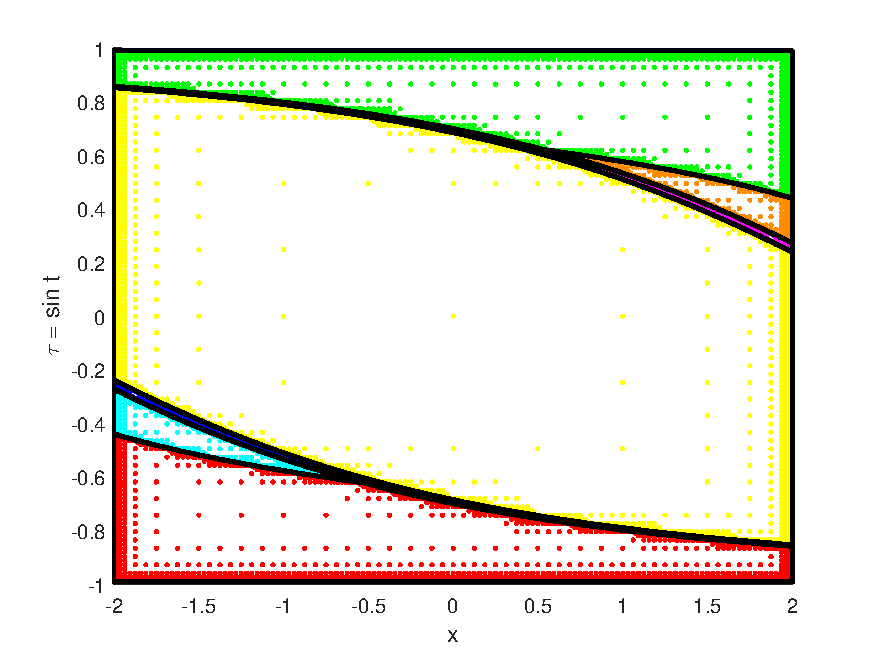
\includegraphics[width=7.7cm]{source1.pdf}
  \end{center}
  \caption{\footnotesize{Distribution of the rays on source phase space. Around $6.9 \cdot 10^4$ rays are traced using the triangulation refinement with parameters:
  $\epsilon_{x_{min}} ~=~ 1 ,$ $ \epsilon_{\tau_{min}} ~=~ 0.5, $ $\epsilon_{x_{max}} ~=~ 3\cdot 10^{-3}, \epsilon_{\tau_{max}} ~=~ 1.5 \cdot 10^{-3}$. Rays that belong to the same region are depicted with the same color. The yellow rays follow the path $\Pi_1 = (1, 2, 7, 12)$;
   the red rays follow the path $\Pi_2 ~= ~(1, 10, 8, 7, 12)$; the green rays follow the path $\Pi_3 = (1, 4, 6, 7, 12)$;
   the blue rays follow the path $\Pi_4= (1, 11, 7, 12)$; the magenta rays follow the path $\Pi_5= (1, 3, 7, 12)$, the cyan rays hit the left detector (line $13$) and follow the path
   $\Pi_6= (1, 10, 7, 8, 13)$ and, the orange rays hit the right detector (line $15$) and follow the path $\Pi_7= (1, 4, 7, 6, 15)$. Each number corresponds to a line of the TIR-collimator as shown in Figure $\ref{fig:analyticlens}$.
  The boundaries are depicted with the black lines.}}
  \label{fig:sourcePS}
\end{figure}


 \begin{figure}[h]
  \begin{center}
  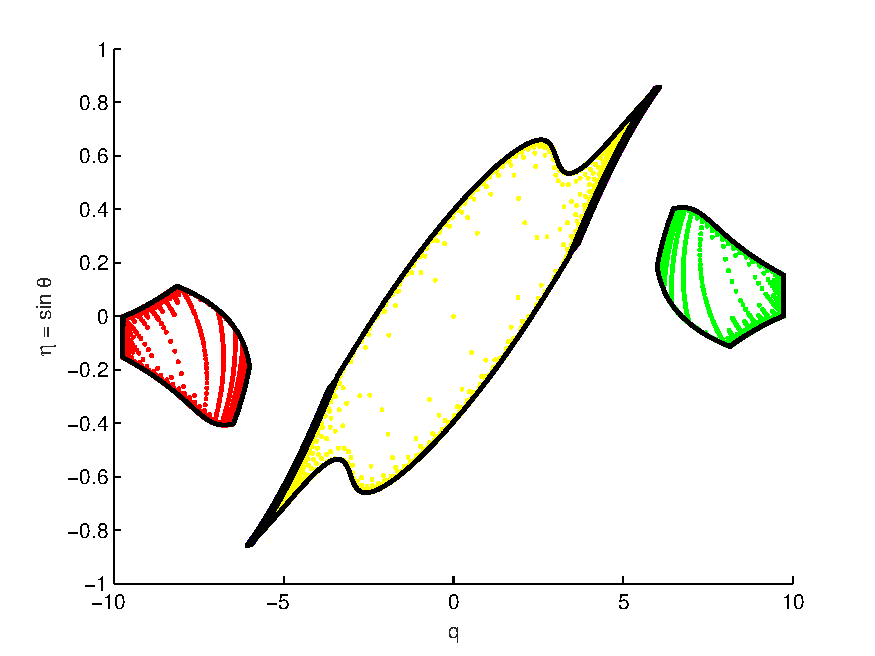
\includegraphics[width=7.7cm]{target.pdf}
  \end{center}
  \caption{\footnotesize{Target phase space representation of a set of $6.9 \cdot 10^4$ rays. Only the rays that hit the target (line $12$) are considered.
  The values of the parameters $\epsilon_{x_{min}}, \epsilon_{x_{max}}, \epsilon_{\tau_{min}}, \epsilon_{\tau_{max}}$ and the choice of the colors for each path are the same as in Figure $\ref{fig:sourcePS}$.
 The boundaries $(\partial R_{\textrm{t}, \Pi_j})_{j = 1, \cdots, p}$ are computed through the triangulation method. The dark areas correspond to areas that are not hit by any meridional plane.}}
  \label{fig:targetPS}
\end{figure}

\indent To conclude, we compute the target intensity which is defined in $\mathcal{P}_{\textrm{t}}$ by Equation (\ref{I(eta)}).
From Equation (\ref{luminance}), we obtain:
\begin{equation}
I_{PS}(\eta) = \sum_{ i, j }\int_{q_{\Pi_j,2i-1}( \eta)}^{q_{\Pi_j, 2i}( \eta)}L_\textrm{t}(q, \eta)\textrm{d}q\,,
\label{eq:Ips}
\end{equation}
where the summation for the indices $i$ is over all $i = 1,2, \cdots, m$, and the summation for the $j$ indices is over all $j$ for which the intersection between $\eta = const$ and $R_{t, \Pi_j}$ is not empty. The intensity is expressed as a function of the angular parameter $\eta~ = ~n_{t}\sin(\theta)$.
In the case of a Lambertian source with $L_{s}(x, \tau) = 1$,
 the following relation for the intensity at the target holds:
\begin{equation}
I_{PS}(\eta) =
\sum_{i,j}(q_{\Pi_j, 2i}(\eta)-q_{\Pi_j,2i-1}(\eta))\,, \label{intensity_eta}
\end{equation}
where the relation  $n_{\textrm{t}}=1$ and conservation of luminance along a ray are exploited, (see \cite{chaves2008introduction}, chapter 16).
We again notice that Equation ($\ref{eq:Ips})$ and (\ref{intensity_eta}) are valid when only two intersection points are found.
If $r>2$ intersection points occur the sum of the distances $(q_{2i}-q_{2i-1})_{i=1, \cdots, m} $ needs to be computed. To calculate the intensity for all the possible directions, a uniform partitioning
$P ~:~ -1\leq \eta_0< \eta_1 \cdots < \eta_{Nb}\leq 1$ of the interval $J = [-1,1]$ is considered, where $Nb= 100$. Eventually, the intensity for each $\eta_h$, with $h = 0,1, \cdots, Nb$, is obtained using relation ($\ref{intensity_eta}$).
  We compare the new method with the already existing MC ray tracing to show its efficiency.\\
 \indent The intensity for MC ray tracing is computed as follows.
 The partitioning $P$ of $J = [-1, 1]$, used for the target phase space, is considered and the number of rays that fall into each bin $([\eta_h, \eta_{h+1}])_{h = 0, \cdots, Nb-1}$ is
 calculated for all $ h \in\{0, \cdots, Nb-1\} $. The intensity in the direction $\eta_k \in [\eta_h, \eta_{h+1}]$ is approximated by:
 \begin{equation}
 \hat{I}_{MC}(\eta_k) = \frac{Nr([\eta_h, \eta_{h+1}])}{Nr([-1, 1])}, \end{equation}
 for every $\Big(\eta_k = \frac{1}{2}(\eta_{h+1}+\eta_h)\Big)_{k = 1,2, \cdots, Nb}$, where we have indicated
 the number of rays that fall into the bin $[\eta_h, \eta_{h+1}]$ with $Nr([\eta_h, \eta_{h+1}])$
 and the total number of rays with $Nr([-1, 1])$. As $\hat{I}_{MC}$  is normalized, a normalization
 of $I_{PS}$ is also required to compare the two intensities.
 This normalization is calculated dividing the intensity by the \'{e}tendue $E_{\mathcal{T}}$ at the target:
 \begin{equation}
 \hat{I}_{PS}(\eta_k) = \frac{1}{E_{\mathcal{T}}} \int_{\eta_h}^{\eta_{h+1}}{I}_{PS}(\eta)\textrm{d}\eta \quad \mbox{for} \quad k = 1,2, \cdots, Nb\,,
 \end{equation}
where ${E_{\mathcal{T}}}$ is obtained by removing the \'{e}tendue corresponding to the regions formed by the rays that hit the left and the right detectors from the total \'{e}tendue $E_{\textrm{t}}$, computed in Equation (\ref{eq:etenduetarget}) and shown in Figure \ref{fig:etendueTS},
Note that the intensities are vectors of length $Nb$, and $\hat{I}_{PS}(\eta_k)_{k = 1,2, \cdots, Nb}$ represent the intensities along the directions $(\eta_k)_{k = 1, \cdots, Nb}$.
The accuracy of the intensity also depends on the number of bins considered in the partitioning $P$.
 Choosing $Nb=100$ results in a smooth profile of the intensity;
 hence, we decide to fix that value of $Nb$.
The photometric variables at the target are now determined for MC and PS method.
The numerical results are shown in the next section.

In this section a comparison between the MC and PS methods is presented.
The MC and PS intensities are calculated several times increasing the number of rays $Nr$ to improve the accuracy.
Both approximate intensities are compared with an intensity taken as a reference.
For some optical systems, there is an explicit solution for the target intensity but this is not the case for the TIR-collimator.
Therefore, the reference intensity $\hat{I}_{\mbox{ref}}$ is obtained considering $1,7 \cdot 10^8$ rays in the MC simulation.
We show how the error,
defined as:
\begin{equation}\label{error}
\mbox{error} = \frac{\sum_{h = 1}^{Nb}| \hat{I}_{PS}(\eta_h) - \hat{I}_{\mbox{ref}}(\eta_h)|}{Nb}\,,
\end{equation}
decreases with the increase in the number of rays.
Table \ref{tab:table} describes how the number of rays traced affects the error estimation and shows the correlation between \'{e}tendue and the number of rays, which is
determined by the values of $\epsilon_{x_{min}}$, $\epsilon_{\tau_{min}}$, $\epsilon_{x_{max}}$ and $\epsilon_{\tau_{max}}$ as explained in Section \ref{sec:method}\ref{subsec:triangulation1}.
 Next, the intensity  $\hat{I}_{MC}$ for the MC method is computed.
Replacing $\hat{I}_{PS}$ with $\hat{I}_{MC}$ in Equation (\ref{error}), the error between the reference intensity and the MC intensity is calculated.
Increasing the number of rays traced in MC ray tracing, the error gradually decreases.
In Table $\ref{tab:table2}$ the numerical results are reported.
\begin{table}[htbp] \label{tab:table}
\centering
\caption{\bf Error values of the PS intensity}
\begin{tabular}{lllll}
 \hline  Number \\ of rays\;   & $\epsilon_{x_{max}} $   \;  & $\epsilon_{\tau_{max}}$\; & \'{e}tendue  & $\mbox{error}$\\
  \hline $1\,403$  & $1.0\cdot 10^{-1}$   & $5.00\cdot 10^{-2}$ & $7.4836$ & $3.57\cdot10^{-4}$ \\
$3\,237$    & $5.0\cdot 10^{-2}$    & $2.50\cdot 10^{-2}$ & $7.6614$ & $2.22\cdot10^{-4}$  \\
$7\,299$   & $2.5 \cdot 10^{-2}$    & $1.25\cdot 10^{-2}$ & $7.7787$ & $1.38\cdot 10^{-4}$ \\
 $15\,919$    & $1.0\cdot 10^{-2}$   & $5.00 \cdot 10^{-3}$ & $7.8475$ & $7.31\cdot 10^{-5}$ \\
 $33\,651$   & $7.0\cdot 10^{-3}$   & $3.50 \cdot 10^{-3}$ & $7.8839$ & $3.80\cdot 10^{-5}$ \\
 $69\,330$  & $3.0\cdot 10^{-3}$    & $1.50 \cdot 10^{-3}$ & $7.9017$ & $2.02\cdot 10^{-5}$ \\
 \hline
 \end{tabular}
 \label{tab:table}
 \end{table}

\begin{table}[htbp]
\centering
\caption{\bf Error values of the MC intensity}
\begin{tabular}{ll} \hline   Number of rays\; & $\mbox{error}_{MC}$\\ \hline $970$  & $2.20\cdot10^{-3}$ \\
$9\,702$  & $6.60\cdot 10^{-4}$  \\ $97\,104$  & $1.74\cdot 10^{-4}$ \\ $971\,436$  & $6.34\cdot 10^{-5}$ \\ $9\,715\,391$  & $2.06\cdot 10^{-5}$ \\
 \hline
 \end{tabular}
 \label{tab:table2}
 \end{table}
\indent The results listed in Table $\ref{tab:table}$ and Table $\ref{tab:table2}$ are shown in Figure $\ref{fig:error}$, where the red line depicts the behavior of the error for the PS
intensity, and the blue line indicates the error for the MC simulation.
\begin{figure}[h!]
  \begin{center}
  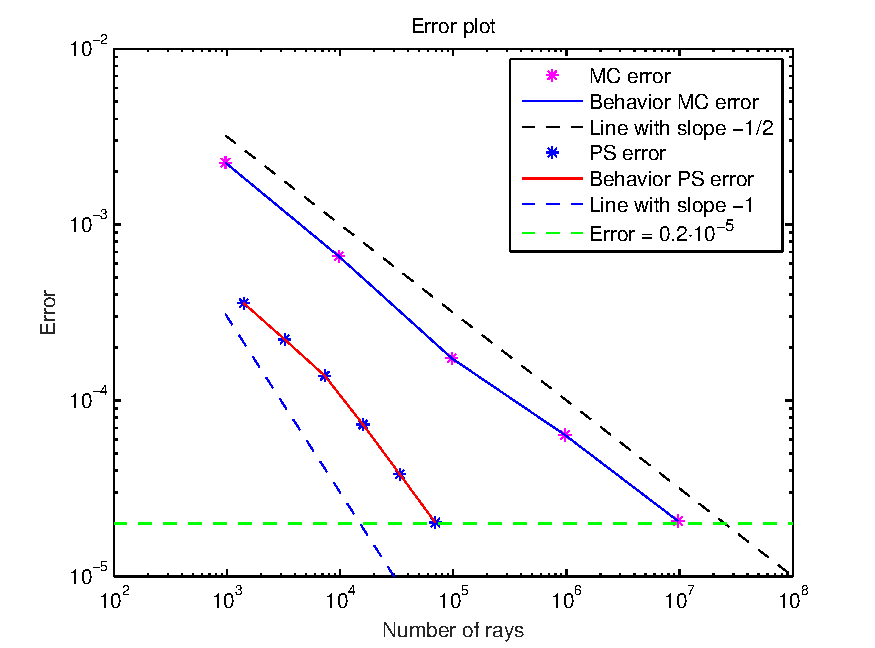
\includegraphics[width=7.7cm]{error.pdf}
  \end{center}
  \caption{\footnotesize{ The red line depicts the error between the intensity on phase space and the reference intensity.
 The blue line shows the error between the Monte Carlo intensity and the reference intensity.
  The dashed black line represents a straight line with the slope equal to $-\frac{1}{2}$.
  The dashed blue line represents a straight line with the slope equal to $-1$.
  The horizontal dotted line shows that an error equal to $2.00 \cdot  10^{-5}$ can be obtained tracing at least $10^2$ times fewer rays in phase space.}}
  \label{fig:error}
\end{figure}
\\
\indent Figure $\ref{fig:error}$ shows that an error equal to $2.00 \cdot  10^{-5}$ is obtained by tracing around $9.7 \cdot 10^{6}$ rays for
MC and only around $6.9 \cdot 10^4$ in PS. The error decreases as $\frac{1}{\sqrt{Nr}}$ for the MC method and as $\frac{1}{Nr}$ for the PS simulation.
  \begin{figure}[h]
    \centering
    \begin{minipage}[]{.40\textwidth}
    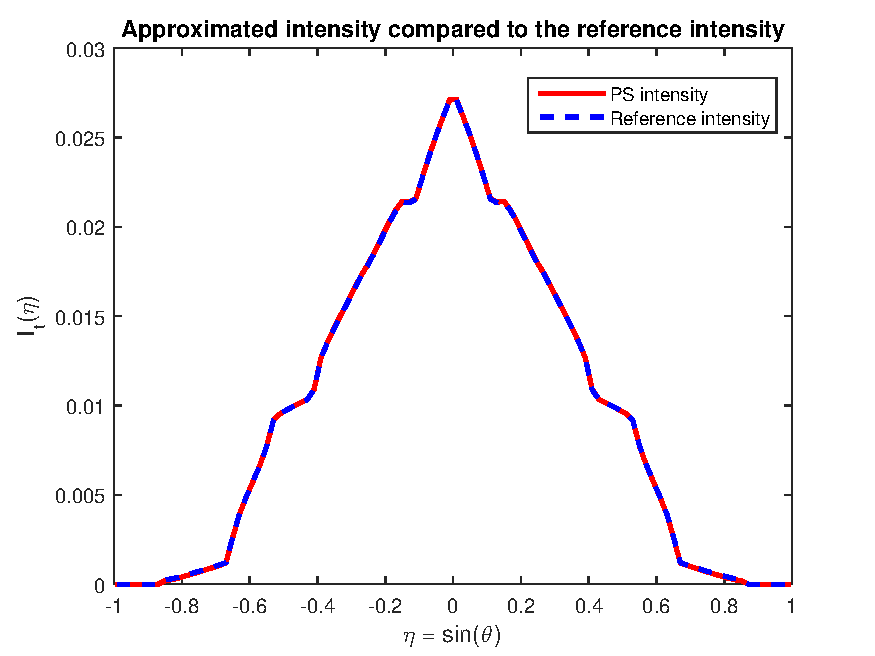
\includegraphics[width=7.7cm]{intensity.pdf}

\caption{\footnotesize{The red line shows the PS intensity at the target of the TIR-collimator. The reference intensity is depicted with the dotted blue line.
The approximate intensity can hardly be distinguished from the exact
intensity. The curves are functions of the angular parameter $\eta = n_{t}\sin(\theta)$. }}
  \label{fig:intensityMCPS}
    \end{minipage} \vspace{2em} \qquad \qquad \qquad
  \end{figure}

\indent The intensity profile $\hat{I}_{PS}(\eta)$ obtained with the phase space method and tracing around $6.9\cdot 10^4$ rays is depicted in Fig. \ref{fig:intensityMCPS} with a red line.
$\hat{I}_{PS}$ is hardly distinguishable from $\hat{I}_{\mbox{ref}}$ (dashed blue line in Figure $\ref{fig:intensityMCPS}$). The intensities are expressed as functions of $\eta$ and thus, the curves in Figure $\ref{fig:intensityMCPS}$ do not depict the spatial intensities.\\
\indent Finally, we claim that PS ray tracing is also more accurate than the ray tracing procedure proposed by Moore (2013), \cite{moore2013methods}.
The novelty of our approach compared to the method used by Moore, is briefly explained below.
First, to compute the output intensity, we employ the phase space of the target. This avoids the use of any interpolation to compute the photometric variables and therefore, more accurate results are obtained.
Second, in \cite{moore2013methods} all rays that leave the source start at the same position and only a sampling angular range is given. In our approach a rectangular source is considered thus, both the angular and spatial coordinates of each ray change. This extra variable can produce very irregular shapes of the regions at target phase space. To overcome this issue, we employ the edge-ray principle and we consider the regions at source phase space where the distribution of the rays is much more regular and the corresponding boundaries are easily computed.
As a consequence, our procedure is suitable to compute the output intensity as function of both the angular or the spatial coordinates.
Third, using the conservation of \'{e}tendue, we provided a criterion to stop the triangulation refinement. In this way we can estimate the number of rays required to obtain the desired accuracy and thus, we avoid tracing more rays than necessary.
\section{Quasi-Monte Carlo method}
